\section{Context-free grammars}

หากกล่าวถึง\emph{ไวยากรณ์} (grammar)s สิ่งแรกที่อาจจะนึกถึงคือ ไวยากรณ์ภาษาอังกฤษ ที่กำหนดวิธีการเขียนประโยคต่างๆ ให้ถูกหลักการ \enskip ตัวอย่างเช่น ลำดับของคำต่อไปนี้เป็นประโยคที่ถูกต้องตามหลักไวยากรณ์ในภาษาอังกฤษ
\[
\str{I think that you believe that he suspects that his girlfriend cheated on him}
\]
หากสังเกตประโยคข้างต้นให้ละเอียดถี่ถ้วน จะเห็นว่า ประโยคดังกล่าวมี\emph{โครงสร้างเวียนบังเกิด} (recursive structure) กล่าวคือ ส่วนท้ายของประโยค (ที่ขึ้นต้นด้วย \str{that} แต่ละตัว) ประกอบด้วยอนุประโยคที่ซ้อนกันโดยไม่จำกัดได้ \enskip ในกรณีทั่วไป ส่วนใดส่วนหนึ่งของประโยคอาจจะแทนที่ได้ด้วยจำนวนคำที่มากขึ้น โดยที่กลุ่มคำเหล่านั้นยังทำให้ถูกหลักไวยากรณ์เหมือนเดิม เช่น จากประโยค \str{I think that you are cute} เราสามารถแทนที่อนุประโยค \str{you are cute} ด้วย \str{I think that you are cute} ได้ กลายเป็น \str{I think that I think that you are cute} ซึ่งยังถูกหลักไวยากรณ์อยู่ และเราสามารถแทนที่แบบนี้ไปได้เรื่อยๆ ไม่มีที่สิ้นสุด

หากจะเขียนไวยากรณ์ภาษาอังกฤษออกมาเป็นกลุ่มของกฎ อาจจะได้ดังรายการต่อไปนี้ ซึ่งทำให้ก่อกำเนิดประโยคในภาษาอังกฤษแบบง่ายๆ ได้ (สังเกตว่า จำนวนประโยคผลลัพธ์ที่เป็นไปได้นั้นมีไม่จำกัด)
\begin{align*}
\ntl{sentence}
 &\to \ntl{noun-phrase}\ntl{verb-phrase} \\
\ntl{noun-phrase}
 &\to \ntl{noun} \\
\ntl{noun-phrase}
 &\to \ntl{adjective}\ntl{noun} \\
\ntl{verb-phrase}
 &\to \ntl{complex-verb} \\
\ntl{verb-phrase}
 &\to \ntl{complex-verb}\ntl{prep-phrase} \\
\ntl{prep-phrase}
 &\to \ntl{prep}\ntl{noun-phrase} \\
\ntl{complex-verb}
 &\to \ntl{verb} \\
\ntl{complex-verb}
 &\to \ntl{verb}\ntl{noun-phrase} \\
\ntl{noun}
 &\to \str{I}\mid\str{you}\mid\str{he}\mid\str{girlfriend}\mid\str{him} \\
\ntl{verb}
 &\to \str{think}\mid\str{believe}\mid\str{suspects}\mid\str{cheated} \\
\ntl{adjective}
 &\to \str{his} \\
\ntl{prep}
 &\to \str{on}\mid\str{that}
\end{align*}
กฎในบรรทัดแรกข้างต้นกล่าวว่า ประโยคใดๆ ประกอบด้วยสองส่วน คือ นามวลี (noun phrase) และกริยาวลี (verb phrase) \enskip กฎที่สองกล่าวว่า นามวลีอาจจะเป็นคำนาม (noun) ได้ ในขณะเดียวกัน กฎข้อที่สามกล่าวว่า นามวลีอาจจะประกอบด้วยคำคุณศัพท์ (adjective) ต่อด้วยคำตามก็ได้ กล่าวคือ นามวลีใดๆ อาจจะเป็นได้สองแบบ \enskip ในส่วนของบุพบทวลี (preposition phrase) นั้น ต้องขึ้นต้นด้วยคำบุพบท (preposition) แล้วตามด้วยนามวลี \enskip สังเกตว่า ในส่วนย่อยๆ ของประโยคนั้น อาจจะอ้างอิงส่วนของประโยคที่เคยใช้มาแล้วก่อนหน้านี้ (ในกรณีของบุพบทวลี สามารถใช้นามวลีเป็นส่วนย่อยได้)

ไวยากรณ์ที่เขียนได้ในลักษณะนี้เรียกว่า\emph{ไวยากรณ์ไม่พึ่งบริบท} (context-free grammar)s

หากต้องการพิจารณาว่าประโยค \str{his girlfriend is cheated on him} นั้นเกิดจากไวยากรณ์ที่กำหนดให้ได้หรือไม่ สามารถเขียนลำดับ\emph{การแปลง} (derivation) ได้ดังนี้
\begin{align*}
\ntl{sentence}
 &\Rightarrow \ntl{noun-phrase}\ \ntl{verb-phrase} \\
 &\Rightarrow \ntl{adjective}\ \ntl{noun}\ \ntl{verb-phrase} \\
 &\Rightarrow \str{his}\ \ntl{noun}\ \ntl{verb-phrase} \\
 &\Rightarrow \str{his}\ \str{girlfriend}\ \ntl{verb-phrase} \\
 &\Rightarrow \str{his}\ \str{girlfriend}\ \ntl{complex-verb}\ \ntl{prep-phrase} \\
 &\Rightarrow \str{his}\ \str{girlfriend}\ \ntl{verb}\ \ntl{prep-phrase} \\
 &\Rightarrow \str{his}\ \str{girlfriend}\ \str{cheated}\ \ntl{prep-phrase} \\
 &\Rightarrow \str{his}\ \str{girlfriend}\ \str{cheated}\ \ntl{prep}\ \ntl{noun-phrase} \\
 &\Rightarrow \str{his}\ \str{girlfriend}\ \str{cheated}\ \str{on}\ \ntl{noun-phrase} \\
 &\Rightarrow \str{his}\ \str{girlfriend}\ \str{cheated}\ \str{on}\ \ntl{noun} \\
 &\Rightarrow \str{his}\ \str{girlfriend}\ \str{cheated}\ \str{on}\ \str{him}
\end{align*}
ในแต่ละขั้นของลำดับการแปลงนั้น เราเลือกส่วนของประโยคที่ยังขยายต่อได้ มาขยายตามกฎใดกฎหนึ่งที่กำหนดไว้ ตัวอย่างเช่น ในการแปลงจากบรรทัดแรกไปยังบรรทัดที่สองข้างต้น เราเลือกขยายส่วนของ \ntl{noun-phrase} ออกเป็น \ntl{adjective}\ntl{noun} โดยใช้กฎข้อที่สามจากไวยากรณ์ก่อนหน้านี้ \enskip ทำเช่นนี้ไปเรื่อยๆ จนกว่าจะไม่มีตัวที่ขยายต่อได้อีก \enskip สังเกตว่า ในลำดับการแปลงข้างต้นนี้ เราเลือกที่จะแปลงสัญลักษณ์ตัวซ้ายสุดที่ยังขยายได้อยู่ การแปลงในลักษณะนี้เรียกว่า\emph{การแปลงจากตัวซ้ายสุด} (leftmost derivation) \enskip ในทางกลับกัน หากเราเลือกแปลงสัญลักษณ์ตัวขวาสุดที่ยังขยายได้อยู่ก่อนเสมอ จะเรียกว่า\emph{การแปลงจากตัวขวาสุด} (rightmost derivation) \enskip หากต้องการเขียน rightmost derivation ของประโยค \str{his girlfriend cheated on him} สามารถเขียนได้ดังนี้
\begin{align*}
\ntl{sentence}
 &\Rightarrow \ntl{noun-phrase}\ \ntl{verb-phrase} \\
 &\Rightarrow \ntl{noun-phrase}\ \ntl{complex-verb}\ \ntl{prep-phrase} \\
 &\Rightarrow \ntl{noun-phrase}\ \ntl{complex-verb}\ \ntl{prep}\ \ntl{noun-phrase} \\
 &\Rightarrow \ntl{noun-phrase}\ \ntl{complex-verb}\ \ntl{prep}\ \ntl{noun} \\
 &\Rightarrow \ntl{noun-phrase}\ \ntl{complex-verb}\ \ntl{prep}\ \str{him} \\
 &\Rightarrow \ntl{noun-phrase}\ \ntl{complex-verb}\ \str{on}\ \str{him} \\
 &\Rightarrow \ntl{noun-phrase}\ \ntl{verb}\ \str{on}\ \str{him} \\
 &\Rightarrow \ntl{noun-phrase}\ \str{cheated}\ \str{on}\ \str{him} \\
 &\Rightarrow \ntl{adjective}\ \ntl{noun}\ \str{cheated}\ \str{on}\ \str{him} \\
 &\Rightarrow \ntl{adjective}\ \str{girlfriend}\ \str{cheated}\ \str{on}\ \str{him} \\
 &\Rightarrow \str{his}\ \str{girlfriend}\ \str{cheated}\ \str{on}\ \str{him}
\end{align*}

อย่างไรก็ดี จะเห็นว่าการเขียน derivation นั้นเกิดความซ้ำซ้อนขึ้น เนื่องจากเราต้องเขียนส่วนของประโยคที่ขยายจนเสร็จสิ้นสมบูรณ์แล้วซ้ำหลายๆ ครั้ง จนกว่าการแปลงจะเสร็จสิ้นสมบูรณ์ทั้งหมด \enskip หากจะลดความซ้ำซ้อน เราสามารถเขียนการแปลงดังกล่าวในรูปของ\emph{ต้นไม้แจงส่วน} (parse tree) ได้ดังรูปที่~\ref{fig:parse-tree}
%
\begin{figure}
\begin{center}
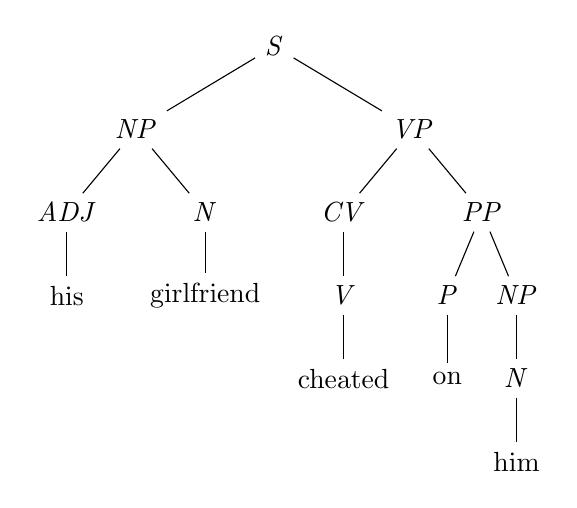
\begin{tikzpicture}[level 1/.style={sibling distance=10em},level 2/.style={sibling distance=5em},level 3/.style={sibling distance=2.5em},level distance=3em]
\node {\textit{S}}
  child {
    node {\textit{NP}}
    child {
      node {\textit{ADJ}}
      child { node {\str{his}} }
    }
    child {
      node {\textit{N}}
      child { node {\str{girlfriend}} }
    }
  }
  child {
    node {\textit{VP}}
    child {
      node {\textit{CV}}
      child {
        node {\textit{V}}
        child { node {\str{cheated}} }
      }
    }
    child {
      node {\textit{PP}}
      child {
        node {\textit{P}}
        child { node {\str{on}} }
      }
      child {
        node {\textit{NP}}
        child {
          node {\textit{N}}
          child { node {\str{him}} }
        }
      }
    }
  }
;
\end{tikzpicture}
\end{center}
\caption{Parse tree for the sentence \str{his girlfriend cheated on him}}
\label{fig:parse-tree}
\end{figure}
%
จะเห็นว่า ส่วนต่างๆ ของประโยคนั้นสามารถเขียนเพียงครั้งเดียวใน parse tree ได้ โดยสามารถอ่านผลลัพธ์ที่ได้จากซ้ายไปขวา \enskip อย่างไรก็ดี การเขียน parse trees ก็ทำให้เราสูญเสียข้อมูลบางอย่างไปด้วย \enskip ในที่นี้ เราไม่สามารถแยกแยะได้ว่า ลำดับการแปลงตั้งแต่ต้นจนจบเป็นอย่างไร อาจจะเป็น leftmost derivation, rightmost derivation, หรือ derivations แบบอื่นก็ได้

ก่อนจะนิยาม context-free grammars เป็นรูปนัย จะขอยกตัวอย่างอีกหนึ่งตัวอย่างก่อน
\begin{example}\label{ex:cfg-0n-sharp-1n}
พิจารณา context-free grammar ต่อไปนี้
\begin{align*}
A &\to \str{0}A\str{1} \\
A &\to B \\
B &\to \str{\#}
\end{align*}
หากเริ่มแปลงจากสัญลักษณ์ $A$ ตัวอย่างของสายอักขระที่เป็นไปได้ รวมถึง parse tree และ leftmost derivation ที่ควบคู่กับสายอักขระแต่ละตัว มีดังนี้
\begin{itemize}
\begin{multicols}{3}
\item \str{0\#1}:
\begin{center}
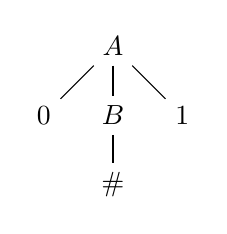
\begin{tikzpicture}[sibling distance=2.5em,level distance=2.5em]
\node {$A$}
  child { node {\str{0}} }
  child {
    node {$B$}
    child { node {\str{\#}} }
  }
  child { node {\str{1}} }
;
\end{tikzpicture}
\end{center}
\begin{align*}
A
 &\Rightarrow \str{0}A\str{1} \\
 &\Rightarrow \str{0}B\str{1} \\
 &\Rightarrow \str{0}\str{\#}\str{1} \\
\end{align*}
\end{multicols}

\begin{multicols}{3}
\item \str{00\#11}:
\begin{center}
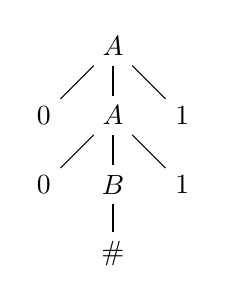
\begin{tikzpicture}[sibling distance=2.5em,level distance=2.5em]
\node {$A$}
  child { node {\str{0}} }
  child {
    node {$A$}
    child { node {\str{0}} }
    child {
      node {$B$}
      child { node {\str{\#}} }
    }
    child { node {\str{1}} }
  }
  child { node {\str{1}} }
;
\end{tikzpicture}
\end{center}
\begin{align*}
A
 &\Rightarrow \str{0}A\str{1} \\
 &\Rightarrow \str{0}\str{0}A\str{1}\str{1} \\
 &\Rightarrow \str{0}\str{0}B\str{1}\str{1} \\
 &\Rightarrow \str{0}\str{0}\str{\#}\str{1}\str{1} \\
\end{align*}
\end{multicols}

\begin{multicols}{3}
\item \str{\#}:
\begin{center}
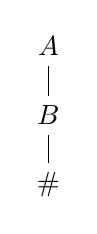
\begin{tikzpicture}[sibling distance=2.5em,level distance=2.5em]
\node {$A$}
  child {
    node {$B$}
    child { node {\str{\#}} }
  }
;
\end{tikzpicture}
\end{center}
\begin{align*}
A
 &\Rightarrow B \\
 &\Rightarrow \str{\#} \\
\end{align*}
\end{multicols}
\end{itemize}

หากพิจารณาให้ถี่ถ้วน จะเห็นว่า grammar นี้\emph{ก่อกำเนิด} (generate)s ภาษา $\set{\str{0}^n\str{\#}\str{1}^n\mid n\geq 0}$ กล่าวคือ เราสามารถเริ่มด้วย \str{\#} ได้ (โดยใช้กฎ $A\to B$) จากนั้น หาก $s$ เป็น string ใดๆ ที่เรามีอยู่แล้ว เราสามารถนำ \str{0} มาปะหน้า และนำ \str{1} มาต่อท้ายไปพร้อมๆ กัน (โดยใช้กฎ $A\to\str{0}A\str{1}$) นั่นคือ จำนวน \str{0} ก่อนหน้า \str{\#} ต้องเท่ากับจำนวน \str{1} ที่อยู่หลัง \str{\#}
\end{example}

ส่วนต่างๆ ของ context-free grammar มีดังนี้
\begin{itemize}
\item สัญลักษณ์ที่เป็นตัวอักษรในสายอักขระ ซึ่งไม่สามารถขยายต่อได้อีก เช่น \str{0} เรียกว่า\emph{สัญลักษณ์ปลายทาง} (terminal symbol)
\item สัญลักษณ์ที่อยู่ในรูปตัวแปร ซึ่งสามารถขยายต่อได้อีก เช่น $A$ เรียกว่า\emph{สัญลักษณ์ระหว่างทาง} (nonterminal symbol)
\item กฎแต่ละตัวที่จะแปลงจาก nonterminal symbol ไปยังส่วนย่อยๆ เช่น $B\to\str{\#}$ เรียกว่า\emph{กฎการผลิต} (production rule)
\end{itemize}

\begin{definition}
\emph{ไวยากรณ์ไม่พึ่งบริบท} (context-free grammar) [CFG] ประกอบด้วย 4 ส่วนดังนี้
\begin{itemize}
\item $V$ เป็นเซตจำกัด (finite set) ของ nonterminal symbols
\item $\Sigma$ เป็น finite set ของ terminal symbols
\item $R$ เป็น finite set ของ production rules ซึ่งแต่ละกฎจะอยู่ในรูป $N\to(V\cup\Sigma)^*$ โดยที่ $N\in V$
\item $S\in V$ เป็น start nonterminal symbol
\end{itemize}

ภาษาที่ก่อกำเนิดได้โดย context-free grammars เรียกว่า\emph{ภาษาไม่พึ่งบริบท} (context-free language)s [CFL]s
\end{definition}
%
\begin{example}
หากเขียน CFG ใน Example~\ref{ex:cfg-0n-sharp-1n} เป็นรูปนัย จะได้ว่า
\begin{itemize}
\item $V=\set{A,B}$
\item $\Sigma=\set{\str{0},\str{1},\str{\#}}$
\item $R=\set{A\to\str{0}A\str{1},A\to B,B\to\str{\#}}$
\item $A$ เป็น start nonterminal symbol
\end{itemize}
\end{example}

ทั้งนี้ หาก nonterminal symbol ใดมี production rules ที่เป็นไปได้หลายตัว สามารถใช้เครื่องหมาย $\mid$ เขียนแยกคั่นกรณีได้ เช่น $A\to\str{0}A\str{1}\mid B$

\begin{example}
พิจารณา $B=\set{\str{0}^n\str{1}^n\mid n\geq 0}$ \enskip หากต้องการพิสูจน์ว่า $B$ เป็น CFL ต้องหา CFG ที่ก่อกำเนิด $B$ \enskip CFG ดังกล่าวสามารถเขียนได้ดังนี้
\begin{align*}
S &\to \str{0}S\str{1} \mid E \\
E &\to \varepsilon
\end{align*}
กล่าวคือ strings ใน $B$ สามารถเป็นได้สองกรณี ในกรณีหลัง เป็น empty string ($\varepsilon$) ได้ ในกรณีแรก หาก string ใดเป็นสมาชิกของ $B$ อยู่แล้ว ก็สามารถนำ \str{0} ปะหน้า และ \str{1} ต่อท้ายในเวลาเดียวกัน โดยผลลัพธ์ที่ได้จะเป็นสมาชิกของ $B$ เหมือนเดิม \enskip หากต้องการเขียน grammar ดังกล่าวโดยใช้ nonterminal symbol เพียงแค่ตัวเดียว สามารถเขียนได้ดังนี้
\[S \to \str{0}S\str{1} \mid \varepsilon\]
\end{example}

\begin{example}
ให้ $\Sigma=\set{\str{a},\str{b}}$ \enskip พิจารณา CFG ต่อไปนี้
\[S \to \str{a}S\str{b} \mid SS \mid \varepsilon\]
หากต้องการหาว่า CFG ดังกล่าวก่อกำเนิดภาษาใด เริ่มแรกอาจจะยังเห็นภาพไม่ชัดเจน ต้องลองเขียน strings บางตัวที่เกิดจาก grammar นี้ได้ก่อน เช่น \str{aaabbb}, \str{abab}, $\varepsilon$, และ \str{aababb} หากพิจารณาให้ถี่ถ้วน จะเห็นว่า strings ในภาษานี้สามารถสร้างได้ 3 วิธี กล่าวคือ
\begin{itemize}
\item หาก $s$ อยู่ในภาษานี้ เราสามารถเติม \str{a} ปะหน้า และ \str{b} ต่อท้าย ก็จะได้ผลลัพธ์ที่ยังอยู่ในภาษานี้ด้วย
\item หาก $s_1$ และ $s_2$ อยู่ในภาษานี้ เราสามารถนำ $s_1$ และ $s_2$ มาต่อกันเป็น $s_1s_2$ ซึ่งก็จะอยู่ในภาษานี้ด้วย
\item $\varepsilon$ อยู่ในภาษานี้
\end{itemize}
แม้ว่าจะพิจารณาแยกกรณีดังกล่าวข้างต้นแล้ว ภาษาที่ต้องการหาอาจจะยังไม่ชัดเจน \enskip หากเปลี่ยน \str{a} แต่ละตัวให้เป็นวงเล็บเปิด \str{(} และ \str{b} แต่ละตัวให้เป็นวงเล็บปิด \str{)} จะได้ว่าตัวอย่าง strings ข้างต้นกลายเป็น \str{((()))}, \str{()()}, $\varepsilon$, และ \str{(()())} ซึ่งสามารถตีความได้เป็น strings ของวงเล็บที่ซ้อนในได้อย่างถูกต้อง (properly nested parentheses) กล่าวคือ strings ในลักษณะนี้สามารถสร้างได้สามวิธีด้วยกัน คือ
\begin{itemize}
\item หาก $s$ เป็นวงเล็บที่ซ้อนในอยู่อย่างถูกต้อง เราสามารถเติม \str{(} ปะหน้า และ \str{)} ต่อท้าย ก็จะได้ผลลัพธ์ที่ยังซ้อนในอย่างถูกต้องเหมือนเดิม
\item หาก $s_1$ และ $s_2$ เป็นวงเล็บที่ซ้อนในอยู่อย่างถูกต้อง เราสามารถนำ $s_1$ และ $s_2$ มาต่อกันเป็น $s_1s_2$ ซึ่งวงเล็บก็ยังซ้อนในได้อย่างถูกต้องเหมือนเดิม
\item $\varepsilon$ มีวงเล็บซ้อนในได้ถูกต้อง เนื่องจากไม่มีวงเล็บเลย เงื่อนไขจึงเป็นจริงโดยปริยาย
\end{itemize}
\end{example}

\begin{example}
หากต้องการเขียน CFG ที่ก่อกำเนิดนิพจน์เลขคณิต (arithmetic expressions) โดยที่ $\Sigma=\set{\str{a},\str{+},\str{*},\str{(},\str{)}}$ สามารถเขียนได้ดังนี้
\[
\begin{array}{ccl}
E
 &\to& E\str{+}E \\
 &\mid& E\str{*}E \\
 &\mid& \str{(}E\str{)} \\
 &\mid& \str{a}
\end{array}
\]
อย่างไรก็ดี หากต้องการ parse \str{a+a*a} จะได้ผลลัพธ์ซึ่งเป็น parse trees มากกว่าหนึ่งแบบ ดังนี้
\begin{center}
\hfill
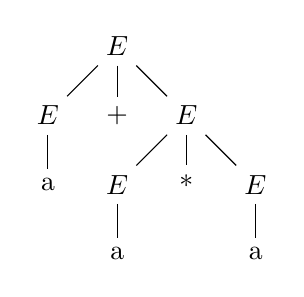
\begin{tikzpicture}[sibling distance=2.5em,level distance=2.5em]
\node {$E$}
  child {
    node {$E$}
    child { node {\str{a}} }
  }
  child { node {\str{+}} }
  child {
    node {$E$}
    child {
      node {$E$}
      child { node {\str{a}} }
    }
    child { node {\str{*}} }
    child {
      node {$E$}
      child { node {\str{a}} }
    }
  }
;
\end{tikzpicture}
%
\hfill
%
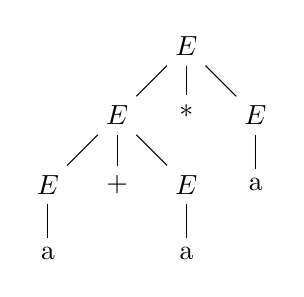
\begin{tikzpicture}[sibling distance=2.5em,level distance=2.5em]
\node {$E$}
  child {
    node {$E$}
    child {
      node {$E$}
      child { node {\str{a}} }
    }
    child { node {\str{+}} }
    child {
      node {$E$}
      child { node {\str{a}} }
    }
  }
  child { node {\str{*}} }
  child {
    node {$E$}
    child { node {\str{a}} }
  }
;
\end{tikzpicture}
\hspace*{\fill}
\end{center}
ในแบบแรก เราทำการบวกเป็นลำดับสุดท้าย เพื่อประกอบ arithmetic expressions ย่อย \str{a} และ \str{a*a} เข้าด้วยกัน \enskip ในแบบหลัง เราทำการคูณเป็นลำดับสุดท้าย เพื่อเชื่อม arithmetic expressions ย่อย \str{a+a} และ \str{a} เข้าด้วยกัน \enskip เนื่องจาก string ดังกล่าวมีหลาย parse trees จึงกล่าวว่า string \str{a+a*a} นี้\emph{แปลงมาอย่างกำกวม} (derived ambiguously) เนื่องจากลำดับการบวกและคูณนั้นไม่กำหนดแน่ชัด \enskip ดังนั้น grammar นี้มีความ\emph{กำกวม} (ambiguous) \enskip นอกจากนี้ string \str{a+a+a} ก็แปลงได้อย่างกำกวมด้วย เนื่องจากเราไม่สามารถกำหนดแน่ชัดได้ว่า จะทำการบวกตัวหน้าหรือตัวหลังก่อน

อย่างไรก็ดี ตามหลักคณิตศาสตร์แล้ว เราควรจะทำการคูณก่อนบวก และบวกตัวซ้ายก่อนตัวขวา \enskip นั่นคือ หากจะประกอบ arithmetic expression ที่ใหญ่ขึ้น ต้องประกอบโดยใช้การบวกหลังการใช้การคูณ และต้องประกอบการบวกตัวซ้ายก่อนที่จะประกอบการบวกตัวขวา ทั้งนี้ หากมีนิพจน์ที่อยู่ในวงเล็บ ต้องประกอบส่วนที่อยู่ในวงเล็บให้เสร็จสิ้นสมบูรณ์ก่อน โดยใช้หลักการเดียวกันกับที่ได้กล่าวมา

จากแนวคิดดังกล่าว เราสามารถทำ\emph{การแก้ไขความกำกวม} (disambiguation) ได้ โดยเขียน CFG ใหม่ที่ยังรับรู้ภาษาเดิม แต่ไม่ทำให้มี strings ที่เขียน parse tree หลายแบบได้ ดังนี้
\begin{align*}
\ntl{expr} &\to \ntl{expr}\str{+}\ntl{term} \mid \ntl{term} \\
\ntl{term} &\to \ntl{term}\str{*}\ntl{factor} \mid \ntl{factor} \\
\ntl{factor} &\to \str{(}\ntl{expr}\str{)} \mid \str{a}
\end{align*}
ในที่นี้ \ntl{expr} คือนิพจน์เลขคณิตทั้งหมดที่เป็นไปได้, \ntl{term} คือนิพจน์เลขคณิตที่ไม่มีเครื่องหมายบวก ยกเว้นจะอยู่ภายในวงเล็บ, และ \ntl{factor} คือนิพจน์เลขคณิตที่ไม่มีเครื่องหมายคูณ ยกเว้นจะอยู่ภายในวงเล็บ \enskip ในที่นี้ ส่วนที่อยู่ในวงเล็บจะเป็น expression อะไรก็ได้ไม่จำกัด \enskip หากใช้ grammar ดังกล่าว \str{a+a*a} จะเหลือเพียง parse tree เดียวดังนี้
\begin{center}
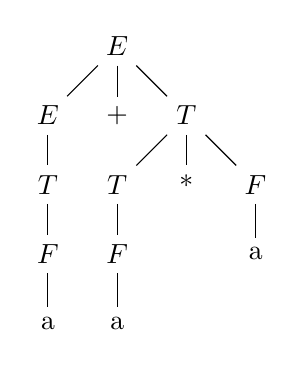
\begin{tikzpicture}[sibling distance=2.5em,level distance=2.5em]
\node {$E$}
  child {
    node {$E$}
    child {
      node {$T$}
      child {
        node {$F$}
        child { node {\str{a}} }
      }
    }
  }
  child { node {\str{+}} }
  child {
    node {$T$}
    child {
      node {$T$}
      child {
        node {$F$}
        child { node {\str{a}} }
      }
    }
    child { node {\str{*}} }
    child {
      node {$F$}
      child { node {\str{a}} }
    }
  }
;
\end{tikzpicture}
\end{center}
\end{example}
ในตัวอย่างข้างต้น เราสามารถเขียน CFG ใหม่ที่ไม่กำกวมได้ อย่างไรก็ดี มี context-free languages ที่ทุกๆ context-free grammar ที่ก่อกำเนิดภาษานั้นๆ ต้องกำกวม \enskip ภาษาในลักษณะนี้เรียกว่ามีความ\emph{กำกวมในตัว} (inherently ambiguous)
%
\begin{example}
$\set{\str{a}^i\str{b}^j\str{c}^k\mid i=j \vee j=k}$ is an inherently ambiguous context-free language.
\end{example}

\begin{exercise}
    เขียน context-free grammar ที่ก่อกำเนิดภาษาข้างต้น แล้วหา string ที่สามารถตีความได้สองวิธีใน grammar ดังกล่าว พร้อมทั้งเขียน parse trees ของการตึความแต่ละวิธีด้วย
\end{exercise}

\begin{example}
อีกตัวอย่างหนึ่งของความกำกวมนั้นเกิดขึ้นในภาษาโปรแกรม (programming languages) \enskip ปัญหานี้เรียกว่า \emph{dangling else} problem ซึ่งมีอยู่ว่า หากเขียนโปรแกรมที่ใช้เงื่อนไขโดยปฏิบัติไม่ครบทุกกรณีในลักษณะนี้
\begin{lstlisting}[language=haskell]
if (b1) then if (b2) then C1 else C2
\end{lstlisting}
ควรจะตีความประโยคดังกล่าวเป็นอย่างไร \enskip ในที่นี้ สามารถตีความได้สองวิธี
\begin{multicols}{2}
\begin{lstlisting}[language=haskell]
if (b1) then {
  if (b2) then
    C1
  else
    C2
}
\end{lstlisting}

\begin{lstlisting}[language=haskell]
if (b1) then {
  if (b2) then
    C1
}
else
  C2
\end{lstlisting}
\end{multicols}
ในวิธีด้านซ้าย ส่วนของ \str{else} ผูกอยู่กับ \str{if} ตัวใน ส่วนในวิธีด้านขวา ส่วนของ \str{else} ผูกอยู่กับ \str{if} ตัวนอก

ปัญหา dangling else เป็นปัญหาเก่าแก่ ที่นักออกแบบภาษาต้องเผชิญและตัดสินใจเลือกตีความประโยคดังกล่าวเป็นอย่างใดอย่างหนึ่ง \enskip ในวงการออกแบบและพัฒนาภาษาโปรแกรมคอมพิวเตอร์ เป็นที่ยอมรับโดยทั่วไปว่าการตีความแบบทางด้านซ้ายจะเหมาะสมกว่า กล่าวคือ \lstinline[language=java]{else} ควรจะคู่กับ \lstinline[language=java]{if} ตัวที่ใกล้ที่สุด หากต้องการเป็นอย่างอื่นควรระบุให้ชัดเจน (เช่น ใส่เครื่องหมายปีกกาคร่อม) \enskip ในที่นี้ เราสามารถเขียน grammar ที่เลือกตีความเป็นแบบแรกได้
\end{example}

ตัวอย่างดังกล่าวเป็นเพียงส่วนหนึ่งของภาษาโปรแกรมเท่านั้น อย่างไรก็ดี programming languages ที่ใช้กันอยู่ในปัจจุบันเกือบทั้งหมดสามารถเขียน\emph{วากยสัมพันธ์} (syntax) เป็น context-free grammars ที่ไม่กำกวมได้

\subsection{Pushdown automata}

ณ จุดนี้ เราได้กล่าวถึง context-free languages และ context-free grammars มาพอสมควร \enskip หากจะย้อนกลับไปเนื้อหาที่เกี่ยวกับ regular languages จะเห็นว่า context-free languages นั้นมีบทบาทในลักษณะเดียวกันกับ regular expressions กล่าวคือ ทั้งสองอย่างนี้ก่อกำเนิดภาษาขึ้นมา \enskip คำถามที่อาจจะตามมาคือ มีกลไกใดหรือไม่ที่รับรู้ context-free languages เช่นเดียวกับที่ finite automata รับรู้ regular languages

กลไกที่รับรู้ context-free languages เรียกว่า \emph{pushdown automata} [PDA] ซึ่งเป็นส่วนต่อขยายมาจาก NFA โดยเพิ่ม\emph{กองซ้อน} (stack) เข้าไป ทำให้สามารถใช้หน่วยความจำได้ไม่จำกัด
%
\begin{example}
PDA ที่รับรู้ $B=\set{\str{0}^n\str{1}^n\mid n\geq 0}$ สามารถเขียนเป็นแผนภาพได้ดังนี้
\begin{center}
\begin{tikzpicture}[node distance=2cm]
\node[initial,state,accepting] (q0) {$q_0$};
\node[state] (q1) [right=of q0] {$q_1$};
\node[state] (q2) [below=of q1] {$q_2$};
\node[state,accepting] (q3) [left=of q2] {$q_3$};

\path[arrow]
  (q0) edge node [above] {$\varepsilon$, $\varepsilon\to\str{\$}$} (q1)
  (q1) edge[loop right] node [right] {\str{0}, $\varepsilon\to\str{0}$} (q1)
       edge node [right] {\str{1}, $\str{0}\to\varepsilon$} (q2)
  (q2) edge[loop right] node [right] {\str{1}, $\str{0}\to\varepsilon$} (q2)
       edge node [above] {$\varepsilon$, $\str{\$}\to\varepsilon$} (q3)
;
\end{tikzpicture}
\end{center}
เริ่มแรก $q_0$ เป็น accept state เนื่องจาก $\varepsilon\in B$ \enskip หลักการของ PDA ดังกล่าวจะนับว่าจำนวน \str{0} มีเท่าจำนวน \str{1} หรือไม่ โดยหากตัวอักษรที่อ่านเข้ามาเป็น \str{0} ให้ push \str{0} ลงใน stack (transition จาก $q_1$ ไป $q_1$ โดยส่วนที่เขียนว่า $\varepsilon\to\str{0}$ หมายความว่า หากด้านบนสุดของ stack ขณะนี้ว่างเปล่า ให้แทนที่ความว่างเปล่าด้วย \str{0} กล่าวคือ push \str{0}) \enskip แต่หากตัวอักษรที่อ่านเข้ามาเป็น \str{1} เราต้องเริ่ม pop stack โดยยังไม่ติดขัดหากยังมี \str{0} ให้เรา pop อยู่ (transitions จาก $q_1$ ไป $q_2$ และ $q_2$ ไป $q_2$ โดยส่วนที่เขียนว่า $\str{0}\to\varepsilon$ หมายความว่า หากด้านบนสุดของ stack เป็น \str{0} ให้แทนที่ด้วยความว่างเปล่า กล่าวคือ หาก pop stack ต้องได้ \str{0} เป็นผลลัพธ์) \enskip เนื่องจากเราไม่สามารถบอกได้ว่า stack ที่ให้มากับ PDA นี้ว่างหรือไม่ จึงต้อง push \str{\$} เข้าไปรองพื้นก่อนเพื่อบ่งบอกว่าก้นของ stack อยู่ ณ ตำแหน่งใด ($\varepsilon$-transition จาก $q_0$ ไป $q_1$) \enskip ในท้ายที่สุด หาก stack นั้นว่างเปล่าแล้ว และเราไม่มีตัวอักษรที่อ่านเพิ่มเติม เราสามารถ pop ตัวรองพื้น \str{\$} แล้วจบการทำงานโดยตอบรับ string ที่ให้มาได้ ($\varepsilon$-transition จาก $q_2$ ไป $q_3$)
\end{example}

\subsection{Non-context-free languages}

ก่อนหน้านี้ เราค้นพบว่า มีภาษาที่ไม่ใช่ regular languages \enskip ในที่นี้ก็เช่นกัน มีภาษาที่ไม่ใช่ context-free languages

\begin{example}
$C=\set{\str{a}^n\str{b}^n\str{c}^n\mid n\geq 0}$ is a non-CFL.
\end{example}

\begin{example}
$F=\set{ww\mid w\in\set{\str{0},\str{1}}^*}$ is a non-CFL.  (สังเกตว่าภาษานี้เป็นภาษาเดียวกันกับ Example~\ref{ex:twice-string-nonreg} ที่เราได้พิสูจน์ไปแล้วว่าไม่ใช่ regular language \enskip ในที่นี้ ภาษานี้ก็ไม่ใช่ context-free language ด้วย)
\end{example}

ในการพิสูจน์ว่าภาษาใดภาษาหนึ่งไม่ใช่ regular language นั้น เราใช้ pumping lemma for regular languages เพื่อหาข้อขัดแย้ง \enskip หากจะพิสูจน์ว่าภาษาหนึ่งๆ ไม่ใช่ context-free language เราก็มี pumping lemma for context-free languages เช่นกันที่สามารถใช้หาข้อขัดแย้งได้ โดยแทนที่จะแบ่ง string ออกเป็นสามส่วน จะต้องแบ่งออกเป็นห้าส่วน โดยที่มีสองส่วนสามารถเขียนซ้ำกี่ครั้งก็ได้
